% -*- Mode:TeX -*-

%% IMPORTANT: The official thesis specifications are available at:
%%            http://libraries.mit.edu/archives/thesis-specs/
%%
%%            Please verify your thesis' formatting and copyright
%%            assignment before submission.  If you notice any
%%            discrepancies between these templates and the 
%%            MIT Libraries' specs, please let us know
%%            by e-mailing thesis@mit.edu

%% The documentclass options along with the pagestyle can be used to generate
%% a technical report, a draft copy, or a regular thesis.  You may need to
%% re-specify the pagestyle after you \include  cover.tex.  For more
%% information, see the first few lines of mitthesis.cls. 

%\documentclass[12pt,vi,twoside]{mitthesis}
%%
%%  If you want your thesis copyright to you instead of MIT, use the
%%  ``vi'' option, as above.
%%
%\documentclass[12pt,twoside,leftblank]{mitthesis}
%%
%% If you want blank pages before new chapters to be labelled ``This
%% Page Intentionally Left Blank'', use the ``leftblank'' option, as
%% above. 

\documentclass[12pt,twoside]{mitthesis}
\usepackage{lgrind}


\usepackage{enumitem}
\usepackage[pdftex]{graphicx}
\usepackage{bbm}
\usepackage{amsfonts}
\usepackage{amsthm}
\usepackage{subfigure}

\theoremstyle{definition}
\newtheorem{defn}{Definition}
\newtheorem{obs}{Observation}
\pagestyle{plain}

%% This bit allows you to either specify only the files which you wish to
%% process, or `all' to process all files which you \include.
%% Krishna Sethuraman (1990).

\typein [\files]{Enter file names to process, (chap1,chap2 ...), or `all' to
process all files:}
\def\all{all}
\ifx\files\all \typeout{Including all files.} \else \typeout{Including only \files.} \includeonly{\files} \fi

\begin{document}

% -*-latex-*-
% 
% For questions, comments, concerns or complaints:
% thesis@mit.edu
% 
%
% $Log: cover.tex,v $
% Revision 1.8  2008/05/13 15:02:15  jdreed
% Degree month is June, not May.  Added note about prevdegrees.
% Arthur Smith's title updated
%
% Revision 1.7  2001/02/08 18:53:16  boojum
% changed some \newpages to \cleardoublepages
%
% Revision 1.6  1999/10/21 14:49:31  boojum
% changed comment referring to documentstyle
%
% Revision 1.5  1999/10/21 14:39:04  boojum
% *** empty log message ***
%
% Revision 1.4  1997/04/18  17:54:10  othomas
% added page numbers on abstract and cover, and made 1 abstract
% page the default rather than 2.  (anne hunter tells me this
% is the new institute standard.)
%
% Revision 1.4  1997/04/18  17:54:10  othomas
% added page numbers on abstract and cover, and made 1 abstract
% page the default rather than 2.  (anne hunter tells me this
% is the new institute standard.)
%
% Revision 1.3  93/05/17  17:06:29  starflt
% Added acknowledgements section (suggested by tompalka)
% 
% Revision 1.2  92/04/22  13:13:13  epeisach
% Fixes for 1991 course 6 requirements
% Phrase "and to grant others the right to do so" has been added to 
% permission clause
% Second copy of abstract is not counted as separate pages so numbering works
% out
% 
% Revision 1.1  92/04/22  13:08:20  epeisach

% NOTE:
% These templates make an effort to conform to the MIT Thesis specifications,
% however the specifications can change.  We recommend that you verify the
% layout of your title page with your thesis advisor and/or the MIT 
% Libraries before printing your final copy.
\title{Modeling Recovery Curves for Prostate Cancer}

\author{Fulton Wang}
% If you wish to list your previous degrees on the cover page, use the 
% previous degrees command:
%       \prevdegrees{A.A., Harvard University (1985)}
% You can use the \\ command to list multiple previous degrees
%       \prevdegrees{B.S., University of California (1978) \\
%                    S.M., Massachusetts Institute of Technology (1981)}
\department{Department of Electrical Engineering and Computer Science}

% If the thesis is for two degrees simultaneously, list them both
% separated by \and like this:
% \degree{Doctor of Philosophy \and Master of Science}
\degree{Masters of Science}

% As of the 2007-08 academic year, valid degree months are September, 
% February, or June.  The default is June.
\degreemonth{June}
\degreeyear{2013}
\thesisdate{May 22, 2013}

%% By default, the thesis will be copyrighted to MIT.  If you need to copyright
%% the thesis to yourself, just specify the `vi' documentclass option.  If for
%% some reason you want to exactly specify the copyright notice text, you can
%% use the \copyrightnoticetext command.  
%\copyrightnoticetext{\copyright IBM, 1990.  Do not open till Xmas.}

% If there is more than one supervisor, use the \supervisor command
% once for each.
\supervisor{Cynthia Rudin}{Assistant Professor}

% This is the department committee chairman, not the thesis committee
% chairman.  You should replace this with your Department's Committee
% Chairman.
\chairman{Leslie Kolodziejski}{Chairman, Department Committee on Graduate Theses}

% Make the titlepage based on the above information.  If you need
% something special and can't use the standard form, you can specify
% the exact text of the titlepage yourself.  Put it in a titlepage
% environment and leave blank lines where you want vertical space.
% The spaces will be adjusted to fill the entire page.  The dotted
% lines for the signatures are made with the \signature command.
\maketitle

% The abstractpage environment sets up everything on the page except
% the text itself.  The title and other header material are put at the
% top of the page, and the supervisors are listed at the bottom.  A
% new page is begun both before and after.  Of course, an abstract may
% be more than one page itself.  If you need more control over the
% format of the page, you can use the abstract environment, which puts
% the word "Abstract" at the beginning and single spaces its text.

%% You can either \input (*not* \include) your abstract file, or you can put
%% the text of the abstract directly between the \begin{abstractpage} and
%% \end{abstractpage} commands.

% First copy: start a new page, and save the page number.
\cleardoublepage
% Uncomment the next line if you do NOT want a page number on your
% abstract and acknowledgments pages.
% \pagestyle{empty}
\setcounter{savepage}{\thepage}
\begin{abstractpage}
% $Log: abstract.tex,v $
% Revision 1.1  93/05/14  14:56:25  starflt
% Initial revision
% 
% Revision 1.1  90/05/04  10:41:01  lwvanels
% Initial revision
% 
%
%% The text of your abstract and nothing else (other than comments) goes here.
%% It will be single-spaced and the rest of the text that is supposed to go on
%% the abstract page will be generated by the abstractpage environment.  This
%% file should be \input (not \include 'd) from cover.tex.
In this thesis, I analyze a dataset containing a time series of various bodily functionality scores for patients following 3 different forms of prostate cancer treatment.  I propose a parametric model for those function level time series and show promise that the method can be applied to both simulated and real data.

\end{abstractpage}

% Additional copy: start a new page, and reset the page number.  This way,
% the second copy of the abstract is not counted as separate pages.
% Uncomment the next 6 lines if you need two copies of the abstract
% page.
% \setcounter{page}{\thesavepage}
% \begin{abstractpage}
% % $Log: abstract.tex,v $
% Revision 1.1  93/05/14  14:56:25  starflt
% Initial revision
% 
% Revision 1.1  90/05/04  10:41:01  lwvanels
% Initial revision
% 
%
%% The text of your abstract and nothing else (other than comments) goes here.
%% It will be single-spaced and the rest of the text that is supposed to go on
%% the abstract page will be generated by the abstractpage environment.  This
%% file should be \input (not \include 'd) from cover.tex.
In this thesis, I analyze a dataset containing a time series of various bodily functionality scores for patients following 3 different forms of prostate cancer treatment.  I propose a parametric model for those function level time series and show promise that the method can be applied to both simulated and real data.

% \end{abstractpage}

\cleardoublepage

\section*{Acknowledgments}

I would like to thank my thesis advisor Cynthia Rudin for her guidance and care, and her willingness to let me join her group.  I would like to thank Tyler McCormick for his cheerful collaboration and insights, Jim Michaelson over at MGH for giving us the medical background we sorely lack.  The small legion of students at MGH provided much needed levity when the data got difficult to work with.  Old labmates - I'm no longer there, but you guys played a big part in my academic development.  Good friends - thanks for supporting me thoughout my journey, and finally, I thank my family for their unwavering faith in me.  

%%%%%%%%%%%%%%%%%%%%%%%%%%%%%%%%%%%%%%%%%%%%%%%%%%%%%%%%%%%%%%%%%%%%%%
% -*-latex-*-

% Some departments (e.g. 5) require an additional signature page.  See
% signature.tex for more information and uncomment the following line if
% applicable.
% % -*- Mode:TeX -*-
%
% Some departments (e.g. Chemistry) require an additional cover page
% with signatures of the thesis committee.  Please check with your
% thesis advisor or other appropriate person to determine if such a 
% page is required for your thesis.  
%
% If you choose not to use the "titlepage" environment, a \newpage
% commands, and several \vspace{\fill} commands may be necessary to
% achieve the required spacing.  The \signature command is defined in
% the "mitthesis" class
%
% The following sample appears courtesy of Ben Kaduk <kaduk@mit.edu> and
% was used in his June 2012 doctoral thesis in Chemistry. 

\begin{titlepage}
\begin{large}
This doctoral thesis has been examined by a Committee of the Department
of Chemistry as follows:

\signature{Professor Jianshu Cao}{Chairman, Thesis Committee \\
   Professor of Chemistry}

\signature{Professor Troy Van Voorhis}{Thesis Supervisor \\
   Associate Professor of Chemistry}

\signature{Professor Robert W. Field}{Member, Thesis Committee \\
   Haslam and Dewey Professor of Chemistry}
\end{large}
\end{titlepage}


\pagestyle{plain}
  % -*- Mode:TeX -*-
%% This file simply contains the commands that actually generate the table of
%% contents and lists of figures and tables.  You can omit any or all of
%% these files by simply taking out the appropriate command.  For more
%% information on these files, see appendix C.3.3 of the LaTeX manual. 
\tableofcontents
\newpage
\listoffigures
\newpage
\listoftables




\chapter{Introduction}

\section{Background}
Prostate cancer is one of the most common cancers, affecting roughly 1 in 5 men in the USA.  Men diagnosed with PC typically have several treatment choices, and to decide between them, one would need to consider what effect the treatment will have on various bodily functions.  For example, radial prostatecomy is known to have a fairly strong effect on sexual function level.  Other bodily functions of interest include urinary, bowel, and general physical function.  To help the patient make their decision, it would be very helpful to provide them with a prediction of what their various function levels would be, should they choose a given treatment.

Typically, each of these functions can be quantified, and are known to change with time.  For example, one can be assigned a sexual function score, and typically one's sexual function score undergoes a steep drop immediately after surgery, before slowly recovering to some steady state level.  Then, the piece of information that would be of use to a patient is to offer them, for each treatment and each function, a \emph{time series} of the function level, should they undergo the given treatment.

Furthermore, data shows that one's function time series for a given treatment varies by patient; different patients undergoing the same treatment should expect to, on average, experience \emph{different} function time series.  For example, patients who are doing poorly in terms of sexual function before surgery should expect to do worse in the long run than patients who were sexually unhealthy before surgery.  

\section{Goal of Project}
Therefore, our goal is to build a predictive model of the \emph{personalized} function time series for patients, taking into account patient attributes such as age, race, comorbidity, and function level prior to treatment.

To help people make decisions, it is not enough to present to a patient a single most likely estimate of their function time series given a treatment - if one is not very certain in the prediction, then that information should be communicated to the patient.  Thus, we will take a Bayesian approach to curve prediction that furthermore utilizes a novel prior structure, reflecting our a priori belief that the more 'extreme' a patient is, the the more uncertainty there would lie in our predictions for a patient.

\section{Desirables for Model}
We would like our model to be Bayesian, because we want to know how much uncertainty there is in our curve predictions.  We want the model to be easily intrepretable -the parameters of our model should have easy to understand meanings.  Finally, we want to build into our model the belief that the 'average' patient should be predicted to have a curve that is the 'average' of all the curves in the dataset.  Without patient-specific predictions, a patient would simply look up a study of prostate cancer, and see on average, how one side effect is affected if he should choose a particular treatment.  In other words, a patient would regard himself as being average, and should expect to have the average response to treatment.  In the case of patient-specific prediction, we believe the average patient should still map to the average curve.  Furthermore, in the absence of data, we should do as before, and predict all patients to have the average response.  This belief will be encoded in the prior distribution for our Bayesian model.  
\chapter{Exploratory Data Analysis}

\section{Dataset}
To build our predictive models, we use a dataset collected by urologists at UCLA, which has previously been used in publication\cite{gore}.  This data follows a cohort of roughly 1000 patients who received one of 3 possible treatments - prostatectomy, radiation therapy, or brachytherapy for a period of 5 years.  Surveys were sent at various time points after treatment that asked patients to assign a functional score in each of several categories: sexual, bowel, and urinary function, as well as general physical and mental well being.  These scores are between 0 and 100.  Several patient attributes such as age, race, comorbidity count, and PSA level were also recorded for every patient.  Figure 1 shows an example of the average sexual function scores in the entire dataset after each of 3 treatments.

\section{General Shape of Function Curves}
The very first thing we did was to see on average what the function curves looked like for different patients, and whether they differed by treatment.  Below, for each of the 3 side effects, we plot the aggregate function time series for patients opting for each treatment.  

\begin{figure}
\centering
\begin{subfigure}[bowel function]{
  \includegraphics[width=.3\linewidth,height=0.3\textheight]{/Users/glareprotector/prostate_git/glare/tex_files/sections/explore/avg_time_series_by_treatment/bowel_func.png}}
\end{subfigure}
\begin{subfigure}[sexual function]{
  \includegraphics[width=.3\linewidth,height=0.3\textheight]{/Users/glareprotector/prostate_git/glare/tex_files/sections/explore/avg_time_series_by_treatment/sexual_func.png}}
\end{subfigure}
\begin{subfigure}[urinary function]{
  \includegraphics[width=.3\linewidth,height=0.3\textheight]{/Users/glareprotector/prostate_git/glare/tex_files/sections/explore/avg_time_series_by_treatment/urin_func.png}}
\end{subfigure}
\caption{Average patient time series for the 3 side effects, stratified by treatment}
\end{figure}

All of the aggregate curves seem to have a similar shape: an initial instantaneous drop off in function level, followed by a rise to some steady state function level.  This hints that we should model the curves parametrically, parameterizing the key attributes of it - the initial drop, the long-term drop, and the rate of function recovery.  Secondly, the treatment chosen does seem to affect the level of initial function drop and long term function level.

\section{Dependence of Function Curves on Patient Attributes}

The second thing we wanted to look at was for a given side effect and treatment, whether the function curves vary depending on the available attributes.  Below, for each of the 3 side effects, for each of the 6 attributes we have for patients, divide the dataset into 2 halves, based on the given attribute.  We plot the average function time series for each half of the dataset, to see if there is a difference.

\begin{figure}
\begin{subfigure}[bowel function]{
  \includegraphics[width=.3\linewidth,height=0.3\textheight]{/Users/glareprotector/prostate_git/glare/tex_files/sections/explore/avg_time_series_strat_by_attribute/bowel_func.png}}
\end{subfigure}
\begin{subfigure}[sexual function]{
  \includegraphics[width=.3\linewidth,height=0.3\textheight]{/Users/glareprotector/prostate_git/glare/tex_files/sections/explore/avg_time_series_strat_by_attribute/sexual_func.png}}
\end{subfigure}
\begin{subfigure}[urinary function]{
  \includegraphics[width=.3\linewidth,height=0.3\textheight]{/Users/glareprotector/prostate_git/glare/tex_files/sections/explore/avg_time_series_strat_by_attribute/urin_func.png}}
\end{subfigure}
\caption{Average patient time series for the 3 side effects, stratified by each of 6 patient attributes}
\end{figure}

It seems like there is a difference in the curves, depending on various attributes.  However, the attributes seem to be strongly correlated with the pre-treatment function level.  It seems logical that the pre-treatment state would be highly correlated with the post-treatment function level.  To verify this, we make the same plots as before, except this time, we stratify the patients by their pre-treatment function level.  Indeed, pre and post-treatment function levels are highly correlated.


\begin{figure}
\begin{subfigure}[bowel function]{
  \includegraphics[width=.3\linewidth,height=0.2\textheight]{/Users/glareprotector/prostate_git/glare/tex_files/sections/explore/avg_time_series_strat_by_pre_state/bowel_func.png}}
\end{subfigure}
\begin{subfigure}[sexual function]{
  \includegraphics[width=.3\linewidth,height=0.2\textheight]{/Users/glareprotector/prostate_git/glare/tex_files/sections/explore/avg_time_series_strat_by_pre_state/sexual_func.png}}
\end{subfigure}
\begin{subfigure}[urinary function]{
  \includegraphics[width=.3\linewidth,height=0.2\textheight]{/Users/glareprotector/prostate_git/glare/tex_files/sections/explore/avg_time_series_strat_by_pre_state/urin_func.png}}
\end{subfigure}
\caption{Average patient time series for the 3 side effects, stratified by each of 6 patient attributes}
\end{figure}


We wonder whether after controlling for the pre-treatment state, a patient's attributes still impact their curves.  Thus, for each side effect, treatment combination, for each of the 6 attributes, we made a scatter plot of the attribute vs the change in side effect function level before treatment and right after treatment (at the 1 month survey time).  There are too many side effect/treatment combinations to display scatter plots for, but below, we choose 3 such combinations and show their associated scatter plots.

\begin{figure}
\begin{subfigure}[bowel function/brachytherapy]{
  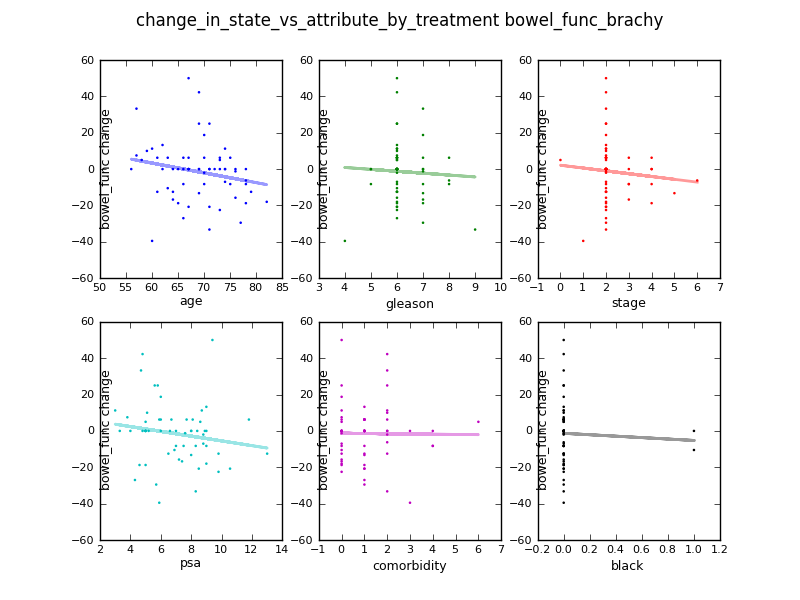
\includegraphics[width=.3\linewidth,height=0.2\textheight]{/Users/glareprotector/prostate_git/glare/tex_files/sections/explore/change_in_state_vs_attribute_by_treatment/bowel_func_brachy.png}}
\end{subfigure}
\begin{subfigure}[sexual function/surgery]{
  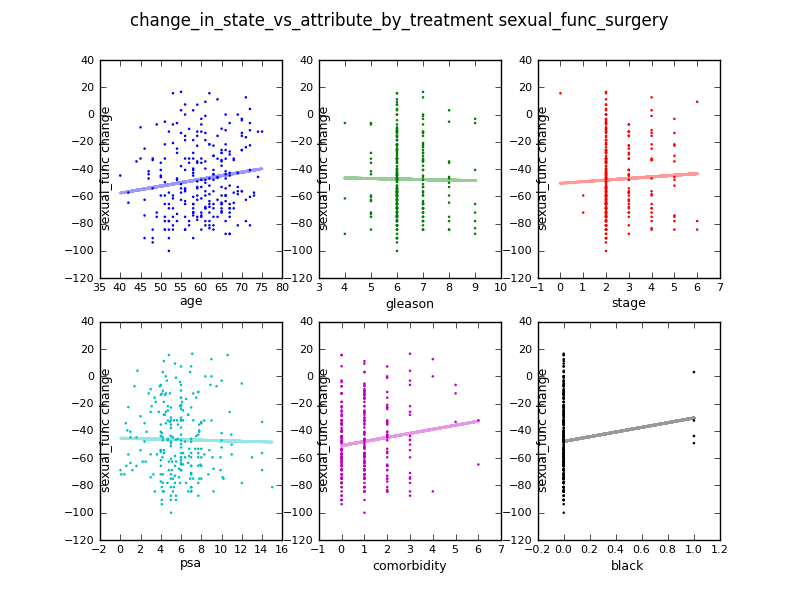
\includegraphics[width=.3\linewidth,height=0.2\textheight]{/Users/glareprotector/prostate_git/glare/tex_files/sections/explore/change_in_state_vs_attribute_by_treatment/sexual_func_surgery.png}}
\end{subfigure}
\begin{subfigure}[urinary function/radiation]{
  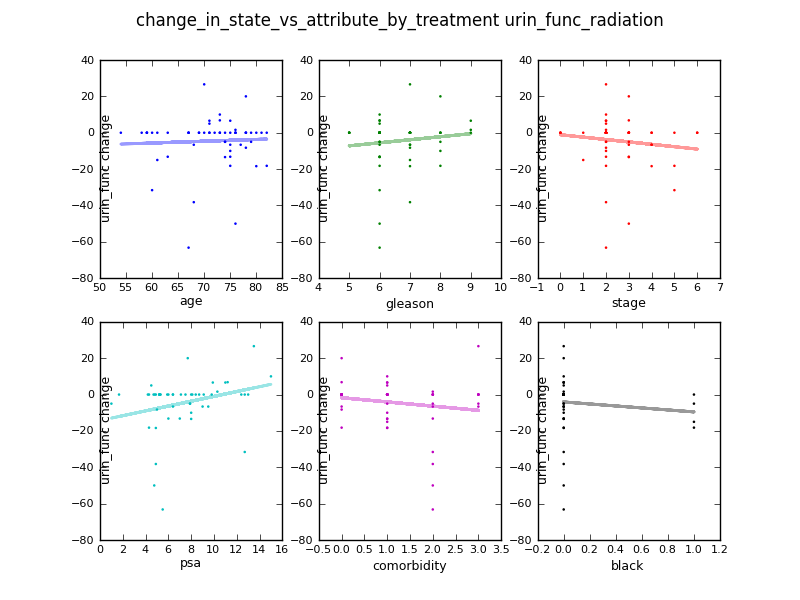
\includegraphics[width=.3\linewidth,height=0.2\textheight]{/Users/glareprotector/prostate_git/glare/tex_files/sections/explore/change_in_state_vs_attribute_by_treatment/urin_func_radiation.png}}
\end{subfigure}
\caption{Initial drop in function level vs attribute, for 3 side effect/treatment combinations}
\end{figure}

There is definitely no trend for some attributes, but perhaps for some there is a slight one.     
\chapter{Model Description}
asdf
\section{Normal Prior}

normal prior

%\end{document}      
\chapter{Curve Prediction with Model}
\section{Bayesian Inference}
The Bayesian approach \cite{gelman}is simple and concise, and after training, ultimately allows us to generate, for a test sample $\tilde{X}$, a distribution over curves $g(t;s,a,b,c,X)$.  In the previous section, we have described a joint distribution over all parameters and data, $P(X,\theta;\alpha)$, where $X$ denotes the observed function value points, and we have integrated out the latent patient curve parameters $a,b,c$.  A patient's curve parameters depend on no other variables besides the parameters $\theta$, if none of the patient's function values are observed, as will be the case when performing prediction.  Thus for a test sample, we need to determine $P(\theta;X,\alpha)$.  Once we have that, we can directly calculate $P(\tilde{a};X,\alpha)=P(\tilde{a};\theta)*P(\theta:X,\alpha)$, and likewise for $\tilde{b}$ and $\tilde{c}$.

To perform the actual inference, we use the standard Metropolis-hastings method\cite{metro}, with our proposals consisting of cycling through the variables of the distribution and proposing to add a normally distributed noise to it.  We use the PYMC package.

\section{Simulation Results}

To show that we can perform posterior inference to extract the posterior distribution of the model parameters $B_a, B_b, B_c$, we simulated data, fixing $B_a, B_b, B_c$.  We simulated 2 different sets of variables.  In both cases, we set $B_a=-1, B_b=1, B_c=2$.  Also, we assume the presence of only 1 covariate, and generated 15 covariates equally spaced in the interval (-2,2) to use as the data $X$.

\subsection{Simulating latent variables $a, b, c$}
In the first scenario, we set $\phi^a=\phi^b=0.5$ and $\phi^c=0.2$, and for each $X_i$, generated $a_i, b_i, c_i$ from the distribution specified by the model.  For example, we generated $a_i$ from a $Beta(B_a*X_i, \phi^a)$ distribution.  This model does not contain any actual function values, since $a,b,c$ are directly simulated/observed.  To perform inference, we used the same model, fixing $\phi^a,\phi^b,\phi^c$ to the values used to generate $a_i,b_i,c_i$, and inferred the distribution of $P(B_a|a_i,b_i,c_i,\phi^a,\phi^b,\phi^c,X_i)$, and likewise for $B_b$ and $B_c$.

\begin{figure}
\centering
\begin{subfigure}{
  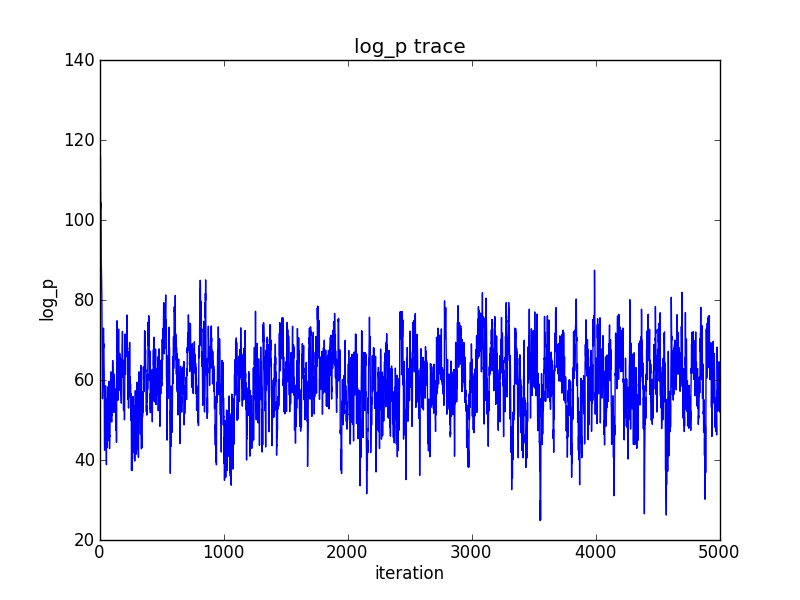
\includegraphics[width=.45\linewidth,height=0.3\textheight]{/Users/glareprotector/prostate_git/glare/tex_files/sections/simulate_data_points_infer_Bs/files/fixing_abc_log_p_trace.png}}
\end{subfigure}
\begin{subfigure}{
  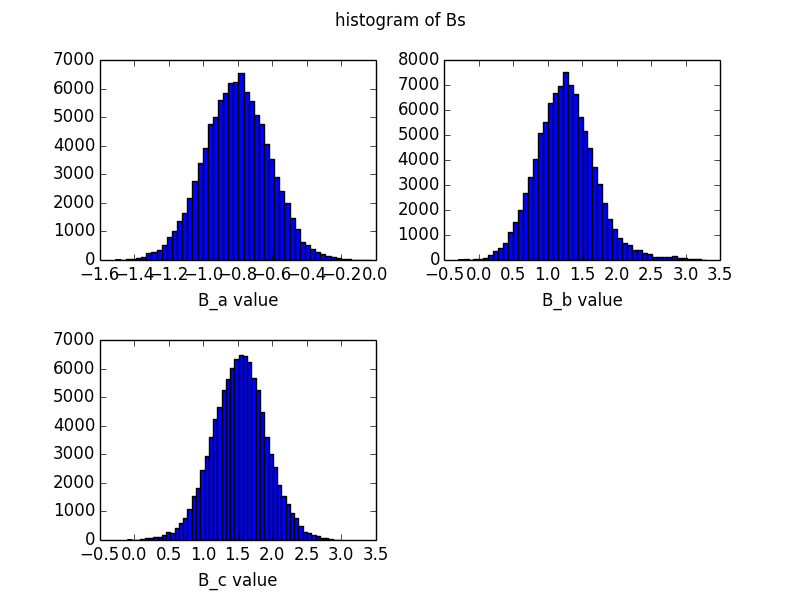
\includegraphics[width=.45\linewidth,height=0.3\textheight]{/Users/glareprotector/prostate_git/glare/tex_files/sections/simulate_data_points_infer_Bs/files/fixing_abc_Bs_histogram.png}}
\end{subfigure}
\begin{subfigure}{
  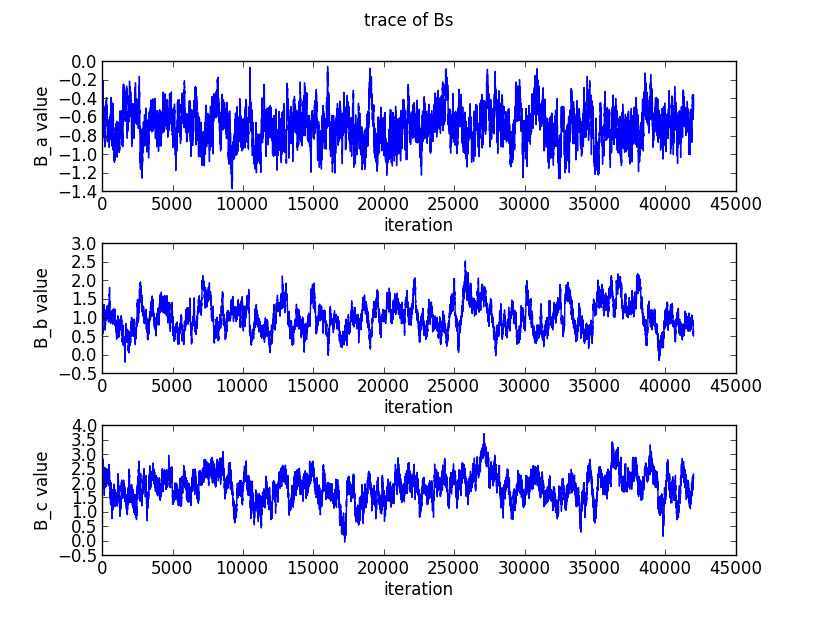
\includegraphics[width=.45\linewidth,height=0.3\textheight]{/Users/glareprotector/prostate_git/glare/tex_files/sections/simulate_data_points_infer_Bs/files/fixing_abc_Bs_trace.png}}
\end{subfigure}
\caption{Plots for when simulating $a,b,c$}
\end{figure}

\subsection{Simulating data points $g^*(t)$}
In the second scenario, we fix the $\phi^a,\phi^b,\phi^c$ and $B_a,B_b,B_c$ as before.  However, we do not simulate $a,b,c$ directly.  Rather, we picked a set of times $t_1 \ldots t_m$, and for each of the 15 patients, simulated $g_i^*(t_j)$ according to the model.  We set $\phi^{noise} = 0.1$.  That is, we first simulate $a_i, b_i, c_i$ and once those are determined, simulate $g_i^*(t_j)$ for each time point $t_j$.  To perform inference of $B_a, B_b, B_c$, we once again assume we know all noise parameters $\phi^a,\phi^b,\phi^c,\phi^{noise}$, and perform sampling to get the distribution of $P(B_a|\{g_i^*(t_j)\},\phi^a,\phi^b,\phi^c,\phi^{noise},X_i)$.

\begin{figure}
\centering
\begin{subfigure}{
  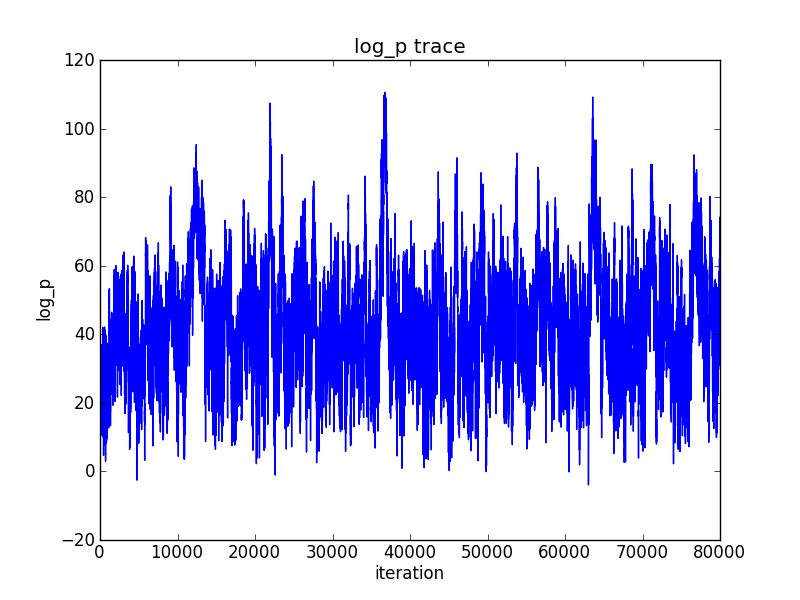
\includegraphics[width=.45\linewidth,height=0.3\textheight]{/Users/glareprotector/prostate_git/glare/tex_files/sections/simulate_data_points_infer_Bs/files/cmatters_log_p_trace.png}}
\end{subfigure}
\begin{subfigure}{
  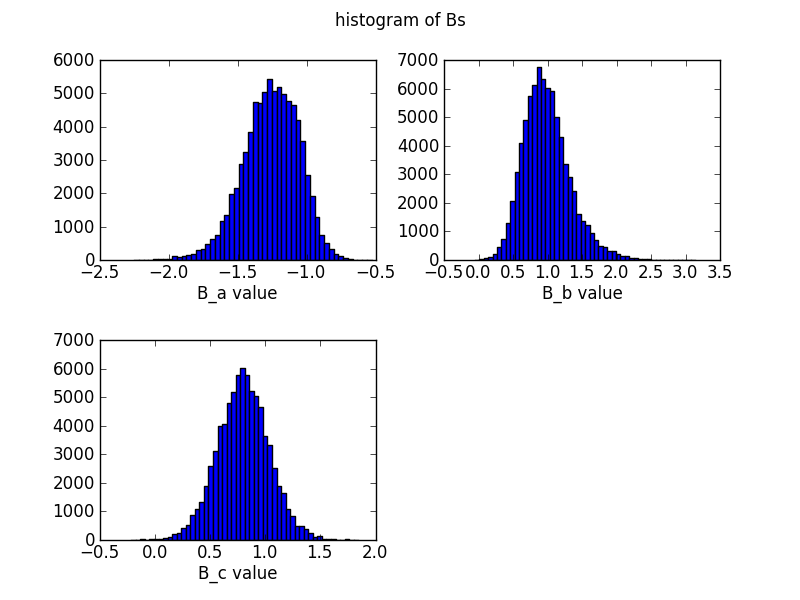
\includegraphics[width=.45\linewidth,height=0.3\textheight]{/Users/glareprotector/prostate_git/glare/tex_files/sections/simulate_data_points_infer_Bs/files/cmatters_Bs_histogram.png}}
\end{subfigure}
\begin{subfigure}{
  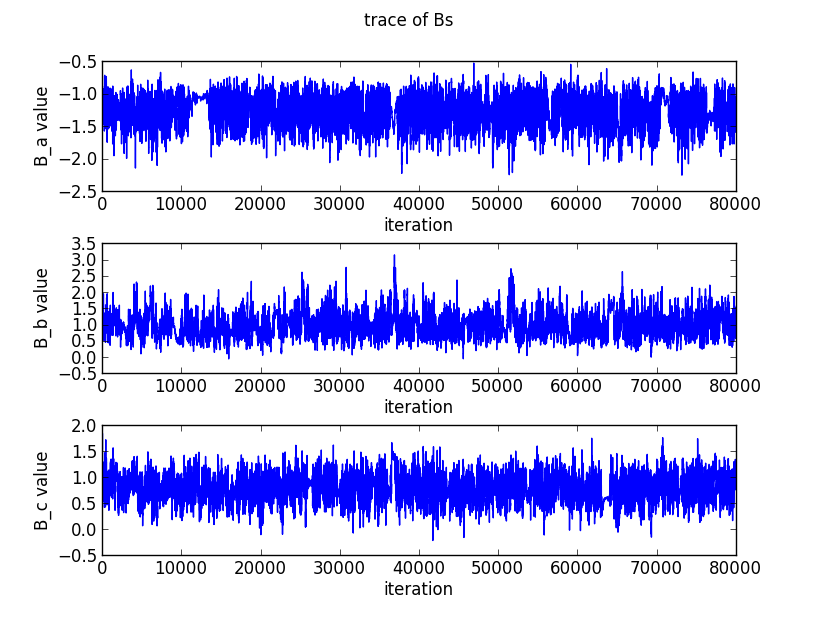
\includegraphics[width=.45\linewidth,height=0.3\textheight]{/Users/glareprotector/prostate_git/glare/tex_files/sections/simulate_data_points_infer_Bs/files/cmatters_Bs_trace.png}}
\end{subfigure}
\caption{Plots for when simulating $a,b,c$}
\end{figure}


\section{Biasedness of model}

From the previous 2 sections, we see that the posterior distributions for $B_a,B_b,B_c$ is actually not centered correctly.  To diagnosis this, I created a simplified model to isolate what was going wrong.  This is basically the part of the model that predicts $a$: 

\begin{eqnarray}
f^a(x) &=& \frac{1}{1+e^{-x}} \\
\mu_i^a &=& f^a(\mu_{pop}^a + B^ax_i) \\
a_i &\sim& Beta(\mu_i^a, \phi^a) \\
B &\sim& U(-\infty,\infty)
\end{eqnarray}

I generate 50 $x_i$'s centered symmetrically about 0.  I set $B_a=1$.  I obtain the corresponding $a_i$'s, with no noise, so that $a_i=\mu_i^a$.  I assume $\phi^a$ is fixed.  I do sampling to infer $P(B_a|a_i,x_i,\phi^a)$.  There is only 1 unobserved variable in this distribution - $B_a$.  The distribution of $P(B_a|a_i,x_i,\phi^a)$ changes as I vary $\phi^a$.  The distribution is centered correctly at 1.0 for small $\phi^a$.  The larger $\phi^a$ is, the more offset the distribution is.  See the following plot.

The reason for this biasedness is that if we fix $\phi^a$ to be large, the distribution for $a_i$ will be U-shaped.  I think posterior for $B_a$ is centered at 0 if $\phi^a$ is close to 1 because when the distribution of $a_i$ is U-shaped, it pays to be off in the predictions.  

\begin{figure}
\centering
\begin{subfigure}[$\phi^a=0.9$]{
  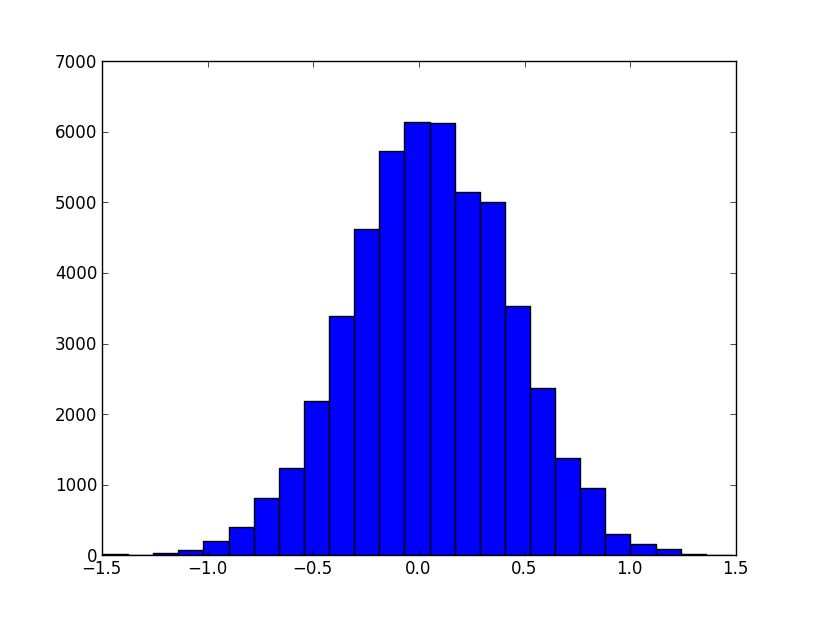
\includegraphics[width=.45\linewidth,height=0.3\textheight]{/Users/glareprotector/Documents/prostate/hist09.png}}
\end{subfigure}
\begin{subfigure}[$\phi^a=0.5$]{
  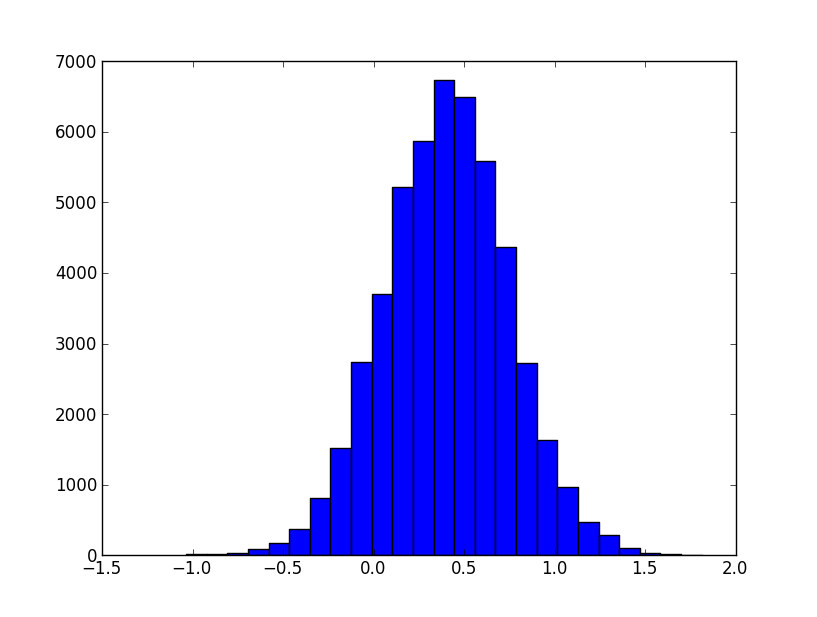
\includegraphics[width=.45\linewidth,height=0.3\textheight]{/Users/glareprotector/Documents/prostate/hist05.png}}
\end{subfigure}
\begin{subfigure}[$\phi^a=0.2$]{
  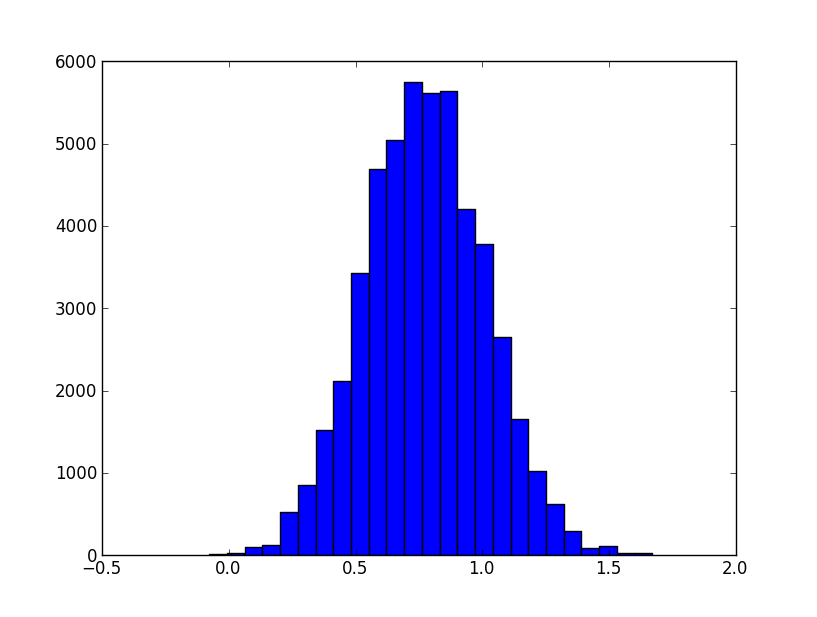
\includegraphics[width=.45\linewidth,height=0.3\textheight]{/Users/glareprotector/Documents/prostate/hist02.png}}
\end{subfigure}
\begin{subfigure}[$\phi^a=0.01$]{
  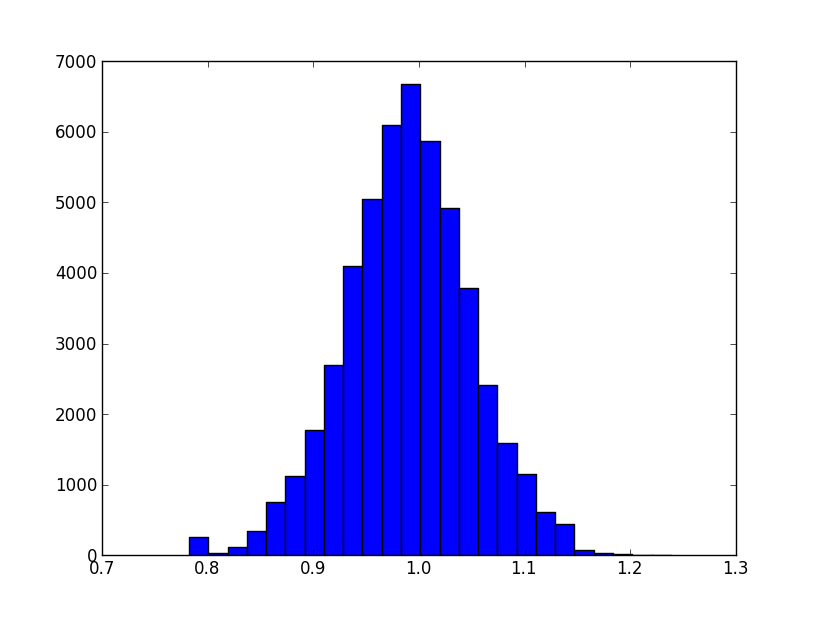
\includegraphics[width=.45\linewidth,height=0.3\textheight]{/Users/glareprotector/Documents/prostate/hist001.png}}
\end{subfigure}
\caption{histogram of posterior of $B_a$ when $\phi^a$ is fixed to various values during inference}
\end{figure}

The solution is to give zero probability to situations where the distribution of $P(a;\mu^a,\phi^a)$ is U-shaped.  This can be done by parameterizing the Beta distributions for $a$ and $b$ differently.  Before, $\phi^a$ represented the proportion of the maximum possible variance for a Beta distribution with the specified mean.  Now, we should let $\phi^a$ represented the proportion of the maximum possible variance for a Beta distribution with the specified mean, such that the distribution is still unimodal.  Hopefully this quantity can be calculated analytically.
\subsection{Applicability of Model to Real Data}
Now that we have parameterized patient function curves, we can explore the relationship between various covariates and curve parameters.  Recall from previous plots that the covariates that seem to affect the curve shape the most are age and the pre-treatment function level.  On the following few pages, for each of the 3 side effect function values, and for each of treatments, and for each of those 2 covariates, we make 4 scatter plots.  For each scatter plot, the x-axis is the covariate, and the y-axis is 1 of 4 curve parameters: $a, b, c$, and also the quantity $a+(1-a)b$, which is equal to the total initial drop in function value, relative to the pre-treatment function value.  This last quantity is labelled as 'drop' in the scatter plots.  Trends in these scatter plots would lead us to believe that the coefficients in the generalized linear models for the $a, b, c$ parameters would be non-zero.

\begin{figure}
\centering
\begin{subfigure}{
  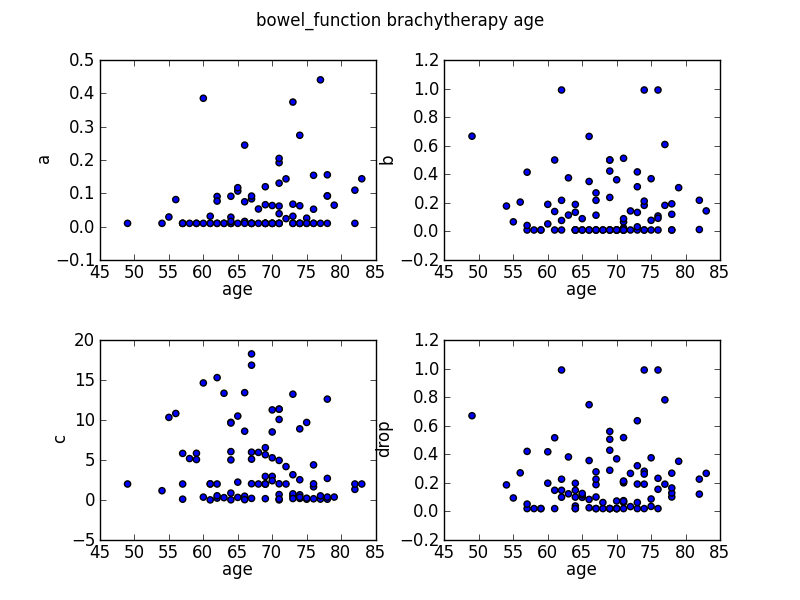
\includegraphics[width=.45\linewidth,height=0.3\textheight]{/Users/glareprotector/prostate_git/glare/tex_files/sections/exploratory_with_abc/files/attribute_vs_curve_parameters/bowel_function_brachytherapy_age.png}}
\end{subfigure}
\begin{subfigure}{
  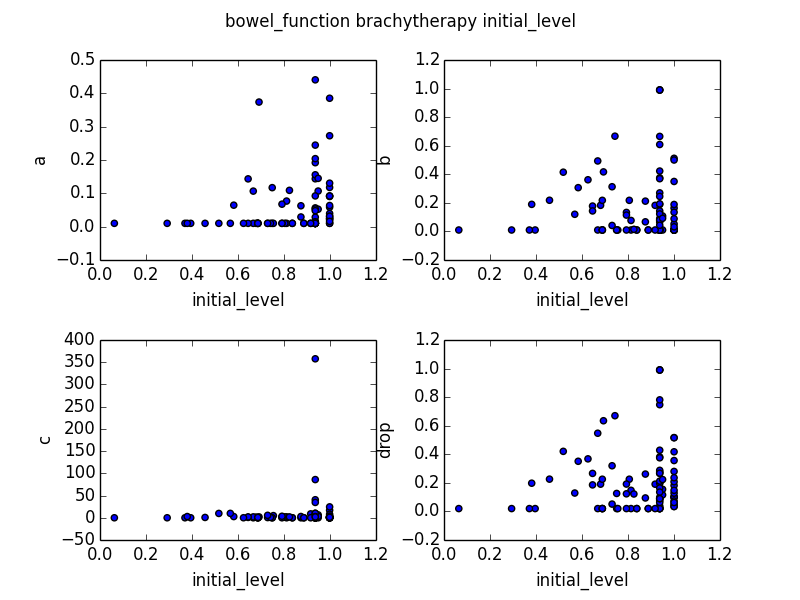
\includegraphics[width=.45\linewidth,height=0.3\textheight]{/Users/glareprotector/prostate_git/glare/tex_files/sections/exploratory_with_abc/files/attribute_vs_curve_parameters/bowel_function_brachytherapy_initial_level.png}}
\end{subfigure}
\begin{subfigure}{
  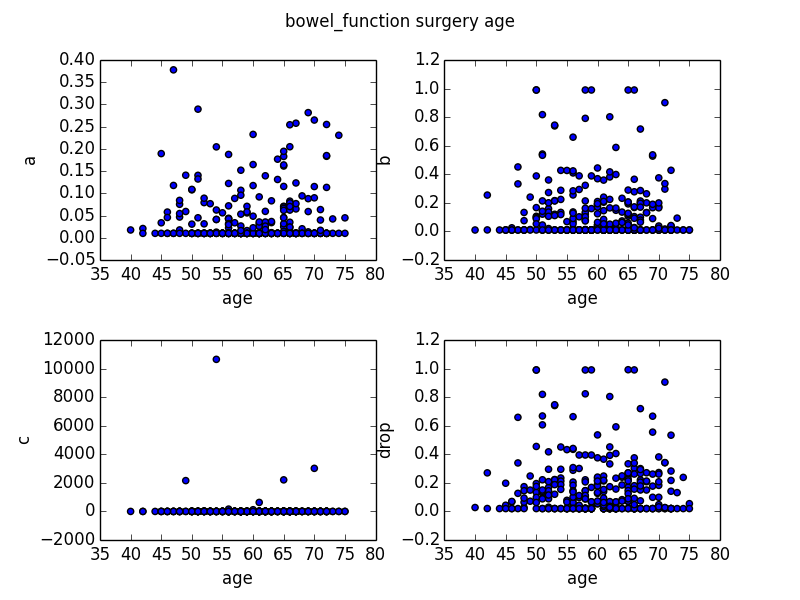
\includegraphics[width=.45\linewidth,height=0.3\textheight]{/Users/glareprotector/prostate_git/glare/tex_files/sections/exploratory_with_abc/files/attribute_vs_curve_parameters/bowel_function_surgery_age.png}}
\end{subfigure}
\begin{subfigure}{
  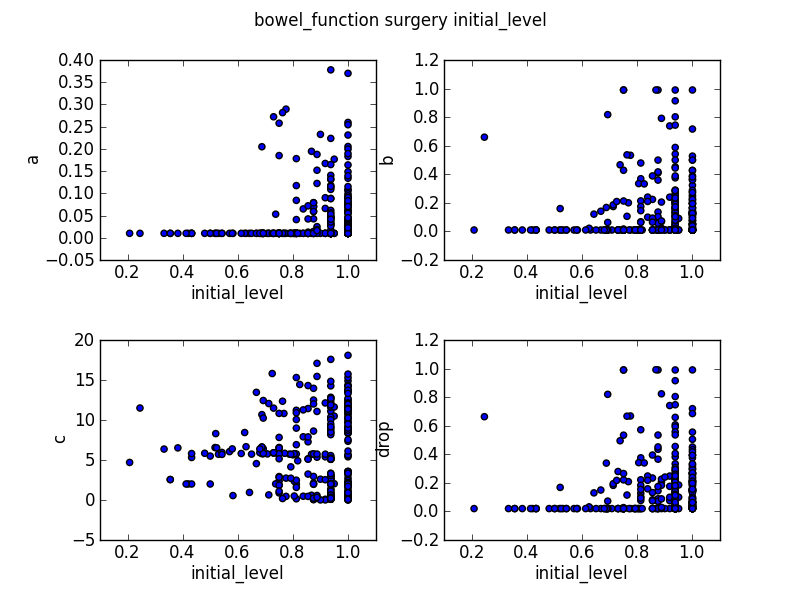
\includegraphics[width=.45\linewidth,height=0.3\textheight]{/Users/glareprotector/prostate_git/glare/tex_files/sections/exploratory_with_abc/files/attribute_vs_curve_parameters/bowel_function_surgery_initial_level.png}}
\end{subfigure}
\begin{subfigure}{
  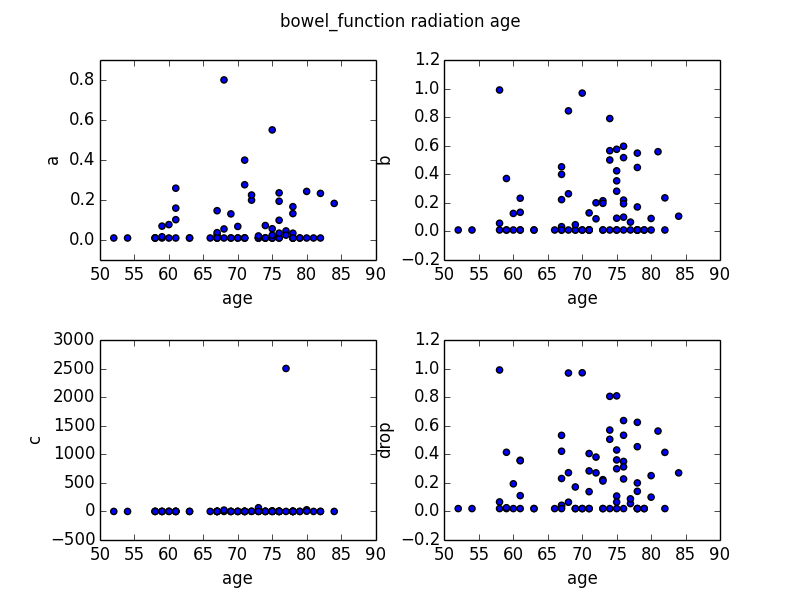
\includegraphics[width=.45\linewidth,height=0.3\textheight]{/Users/glareprotector/prostate_git/glare/tex_files/sections/exploratory_with_abc/files/attribute_vs_curve_parameters/bowel_function_radiation_age.png}}
\end{subfigure}
\begin{subfigure}{
  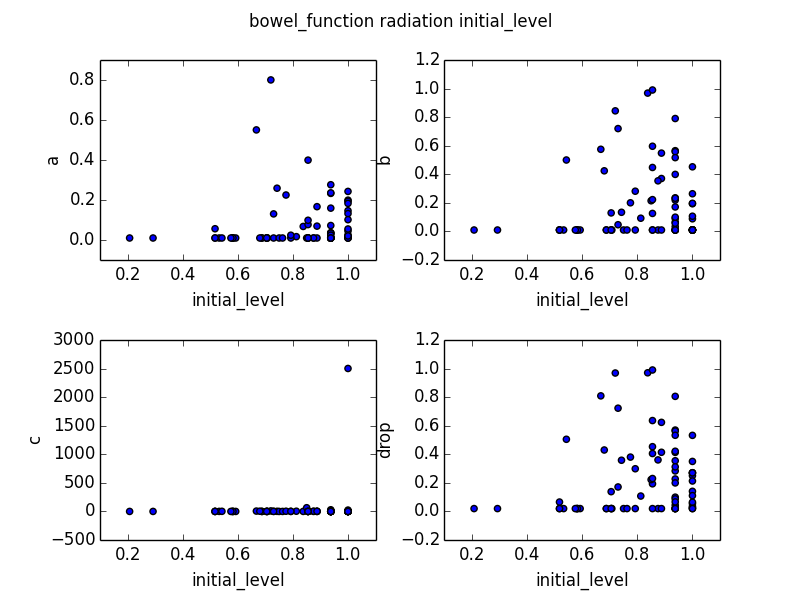
\includegraphics[width=.45\linewidth,height=0.3\textheight]{/Users/glareprotector/prostate_git/glare/tex_files/sections/exploratory_with_abc/files/attribute_vs_curve_parameters/bowel_function_radiation_initial_level.png}}
\end{subfigure}
\caption{Plots of bowel function curve parameters vs initial function level and age attribute, stratified by treatment}
\end{figure}

\begin{figure}
\centering
\begin{subfigure}{
  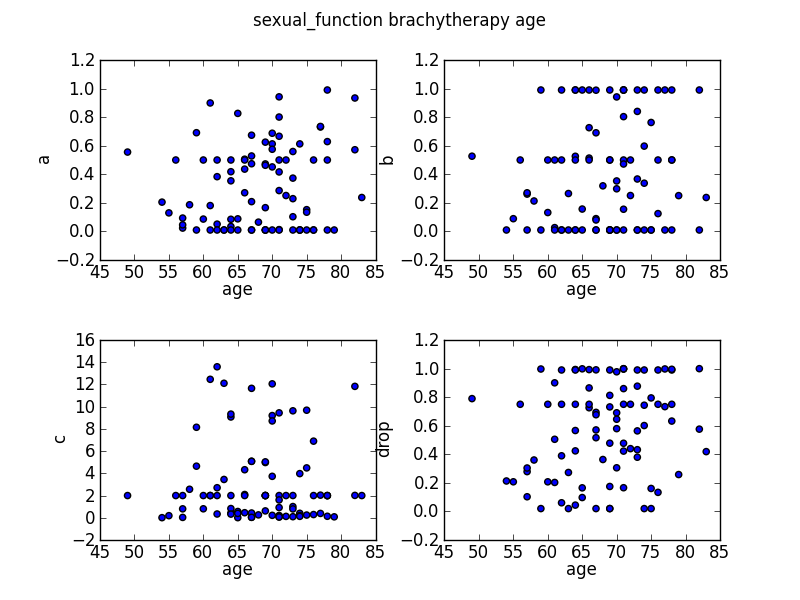
\includegraphics[width=.45\linewidth,height=0.3\textheight]{/Users/glareprotector/prostate_git/glare/tex_files/sections/exploratory_with_abc/files/attribute_vs_curve_parameters/sexual_function_brachytherapy_age.png}}
\end{subfigure}
\begin{subfigure}{
  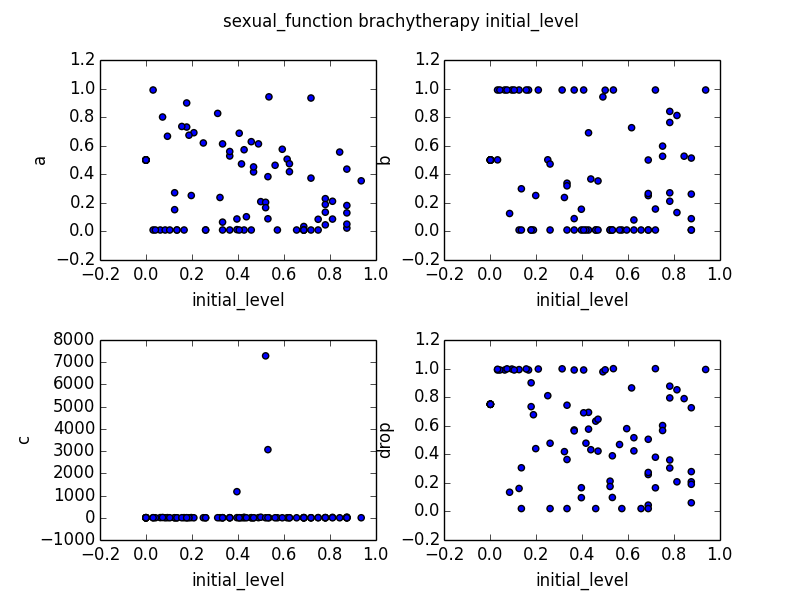
\includegraphics[width=.45\linewidth,height=0.3\textheight]{/Users/glareprotector/prostate_git/glare/tex_files/sections/exploratory_with_abc/files/attribute_vs_curve_parameters/sexual_function_brachytherapy_initial_level.png}}
\end{subfigure}
\begin{subfigure}{
  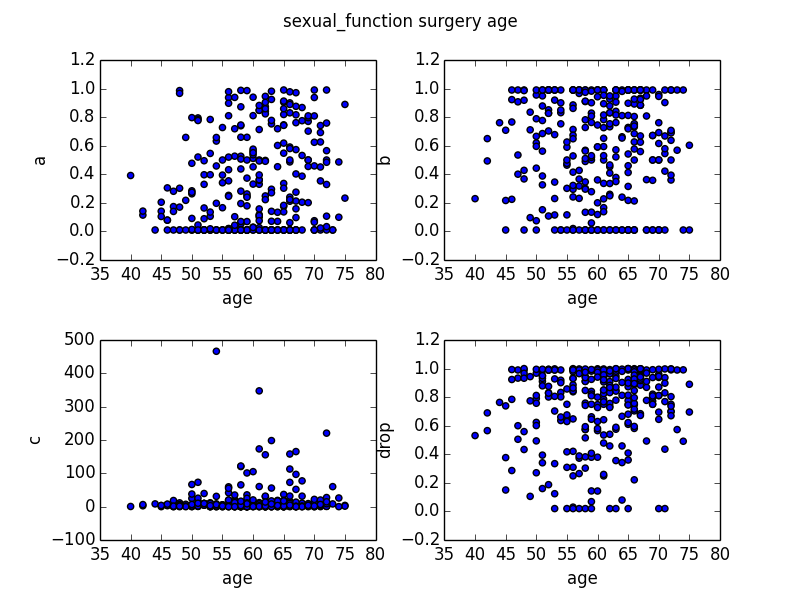
\includegraphics[width=.45\linewidth,height=0.3\textheight]{/Users/glareprotector/prostate_git/glare/tex_files/sections/exploratory_with_abc/files/attribute_vs_curve_parameters/sexual_function_surgery_age.png}}
\end{subfigure}
\begin{subfigure}{
  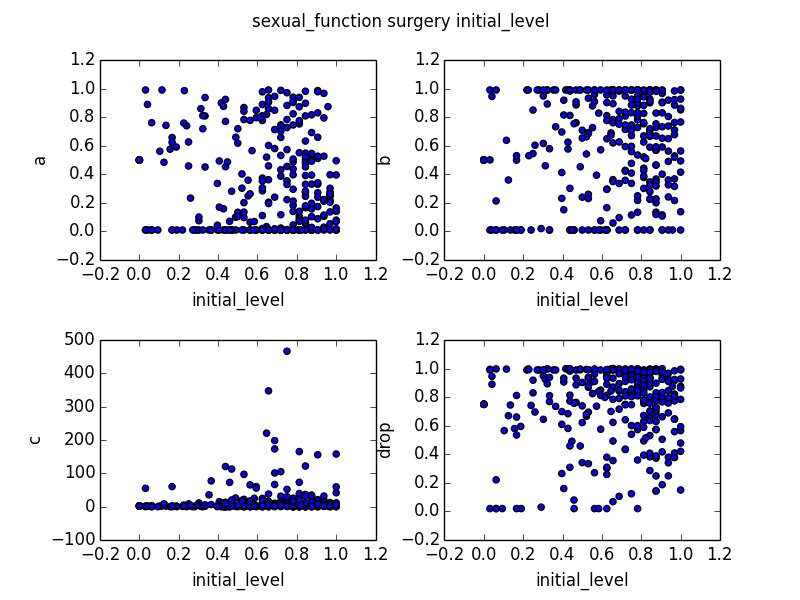
\includegraphics[width=.45\linewidth,height=0.3\textheight]{/Users/glareprotector/prostate_git/glare/tex_files/sections/exploratory_with_abc/files/attribute_vs_curve_parameters/sexual_function_surgery_initial_level.png}}
\end{subfigure}
\begin{subfigure}{
  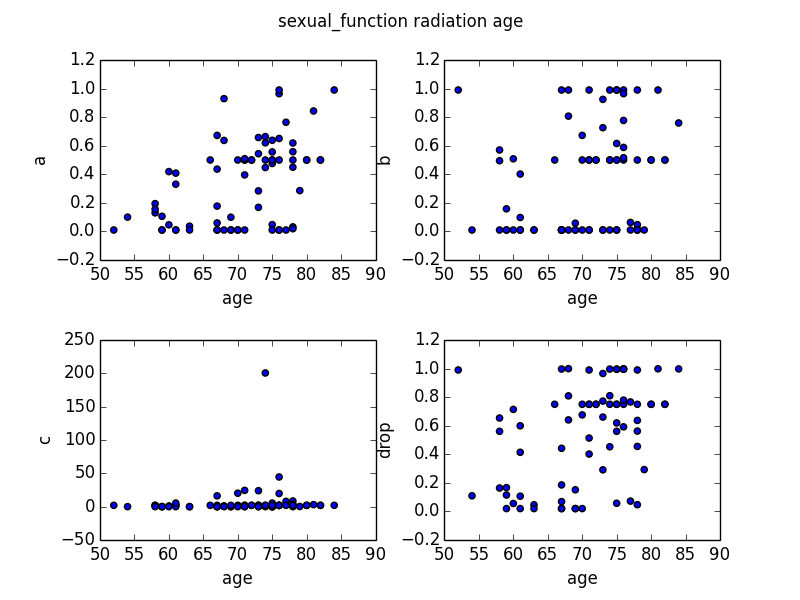
\includegraphics[width=.45\linewidth,height=0.3\textheight]{/Users/glareprotector/prostate_git/glare/tex_files/sections/exploratory_with_abc/files/attribute_vs_curve_parameters/sexual_function_radiation_age.png}}
\end{subfigure}
\begin{subfigure}{
  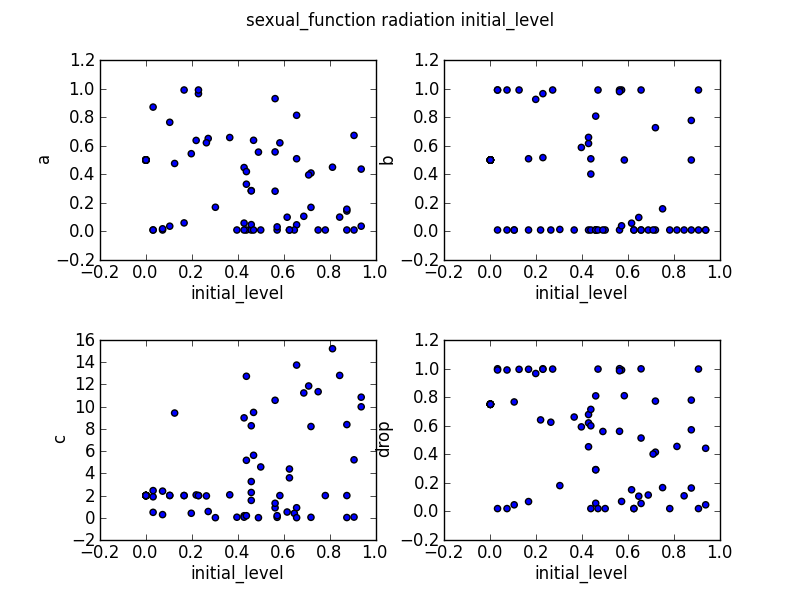
\includegraphics[width=.45\linewidth,height=0.3\textheight]{/Users/glareprotector/prostate_git/glare/tex_files/sections/exploratory_with_abc/files/attribute_vs_curve_parameters/sexual_function_radiation_initial_level.png}}
\end{subfigure}
\caption{Plots of sexual function curve parameters vs initial function level and age attribute, stratified by treatment}
\end{figure}

\begin{figure}
\centering
\begin{subfigure}{
  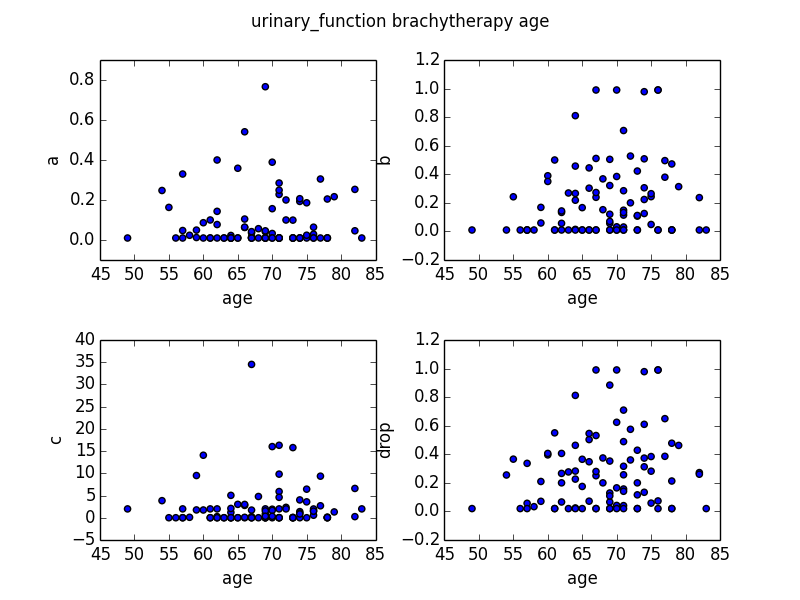
\includegraphics[width=.45\linewidth,height=0.3\textheight]{/Users/glareprotector/prostate_git/glare/tex_files/sections/exploratory_with_abc/files/attribute_vs_curve_parameters/urinary_function_brachytherapy_age.png}}
\end{subfigure}
\begin{subfigure}{
  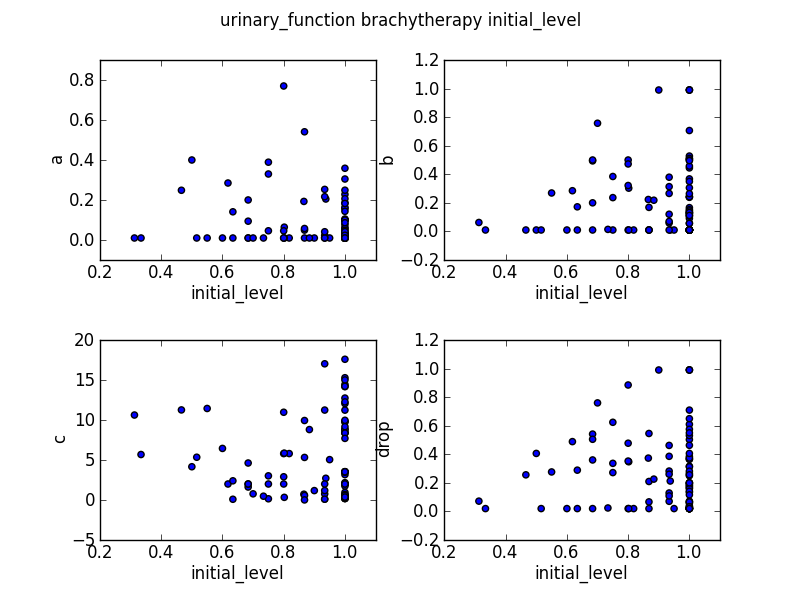
\includegraphics[width=.45\linewidth,height=0.3\textheight]{/Users/glareprotector/prostate_git/glare/tex_files/sections/exploratory_with_abc/files/attribute_vs_curve_parameters/urinary_function_brachytherapy_initial_level.png}}
\end{subfigure}
\begin{subfigure}{
  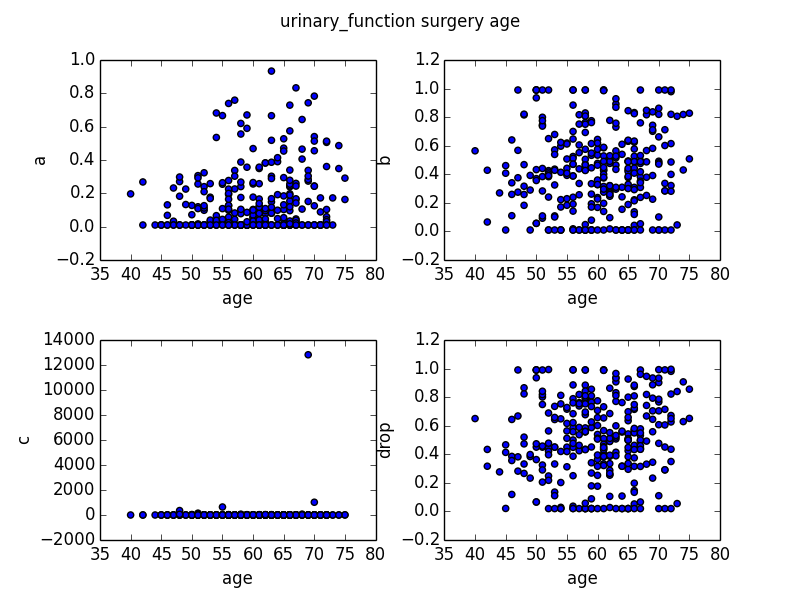
\includegraphics[width=.45\linewidth,height=0.3\textheight]{/Users/glareprotector/prostate_git/glare/tex_files/sections/exploratory_with_abc/files/attribute_vs_curve_parameters/urinary_function_surgery_age.png}}
\end{subfigure}
\begin{subfigure}{
  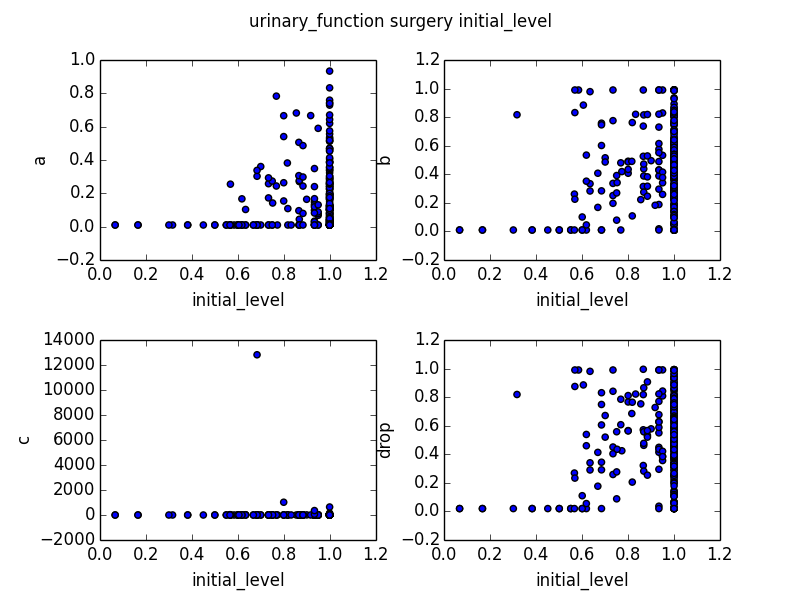
\includegraphics[width=.45\linewidth,height=0.3\textheight]{/Users/glareprotector/prostate_git/glare/tex_files/sections/exploratory_with_abc/files/attribute_vs_curve_parameters/urinary_function_surgery_initial_level.png}}
\end{subfigure}
\begin{subfigure}{
  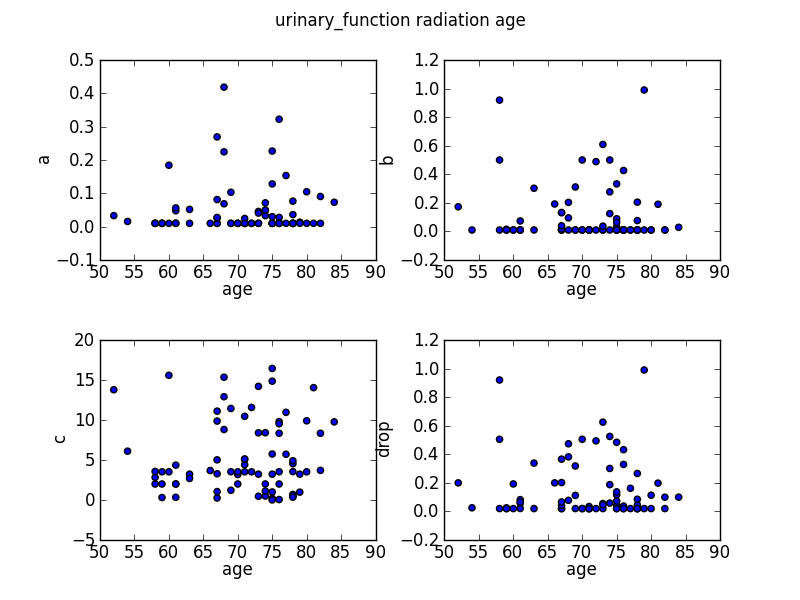
\includegraphics[width=.45\linewidth,height=0.3\textheight]{/Users/glareprotector/prostate_git/glare/tex_files/sections/exploratory_with_abc/files/attribute_vs_curve_parameters/urinary_function_radiation_age.png}}
\end{subfigure}
\begin{subfigure}{
  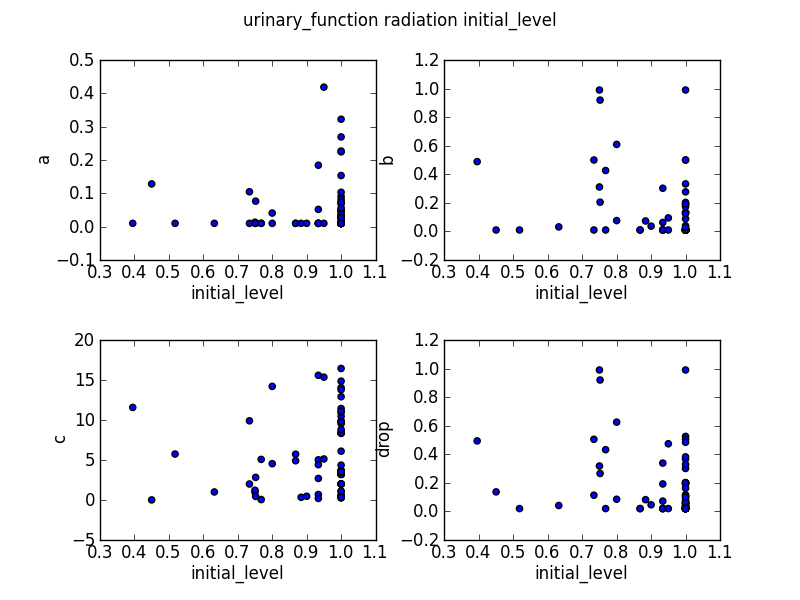
\includegraphics[width=.45\linewidth,height=0.3\textheight]{/Users/glareprotector/prostate_git/glare/tex_files/sections/exploratory_with_abc/files/attribute_vs_curve_parameters/urinary_function_radiation_initial_level.png}}
\end{subfigure}
\caption{Plots of sexual function curve parameters vs initial function level and age attribute, stratified by treatment}
\end{figure}      


\begin{thebibliography}{9}
\bibitem{smithson} Smithson M, Verkuilen J.  A Better Lemon Squeezer, Maximum-Likelihood Regression with Beta-Distributed Dependent Variables.  Psychological Methods.   2006.
\bibitem{gore} Gore J, Kwan L, Lee S, Reiter R, Litwin M.  Survivorship Beyond Convalescence: 48-Month Quality-Of-Life Outcomes after Treatment for Localized Prostate Cancer.  J Natl Cancer Inst.  2009.
\bibitem{gelman} Gelman A.  Bayesian Data Analysis.  2003.
\bibitem{metro}  Metropolis N, Rosenbluth A, Rosenbluth M.  Equations of State Calculations by Fast Computing Machines.  Journal of Chemical Physics.  1953.
\end{thebibliography}
\end{document}

